\chapter{Longitude and Latitude}

\section{Longitude and Latitude}
The Earth can be represented as a sphere, and the position of a point
on its surface can be described using two coordinates: latitude and
longitude.

\begin{figure}[htbp]
    \centering
    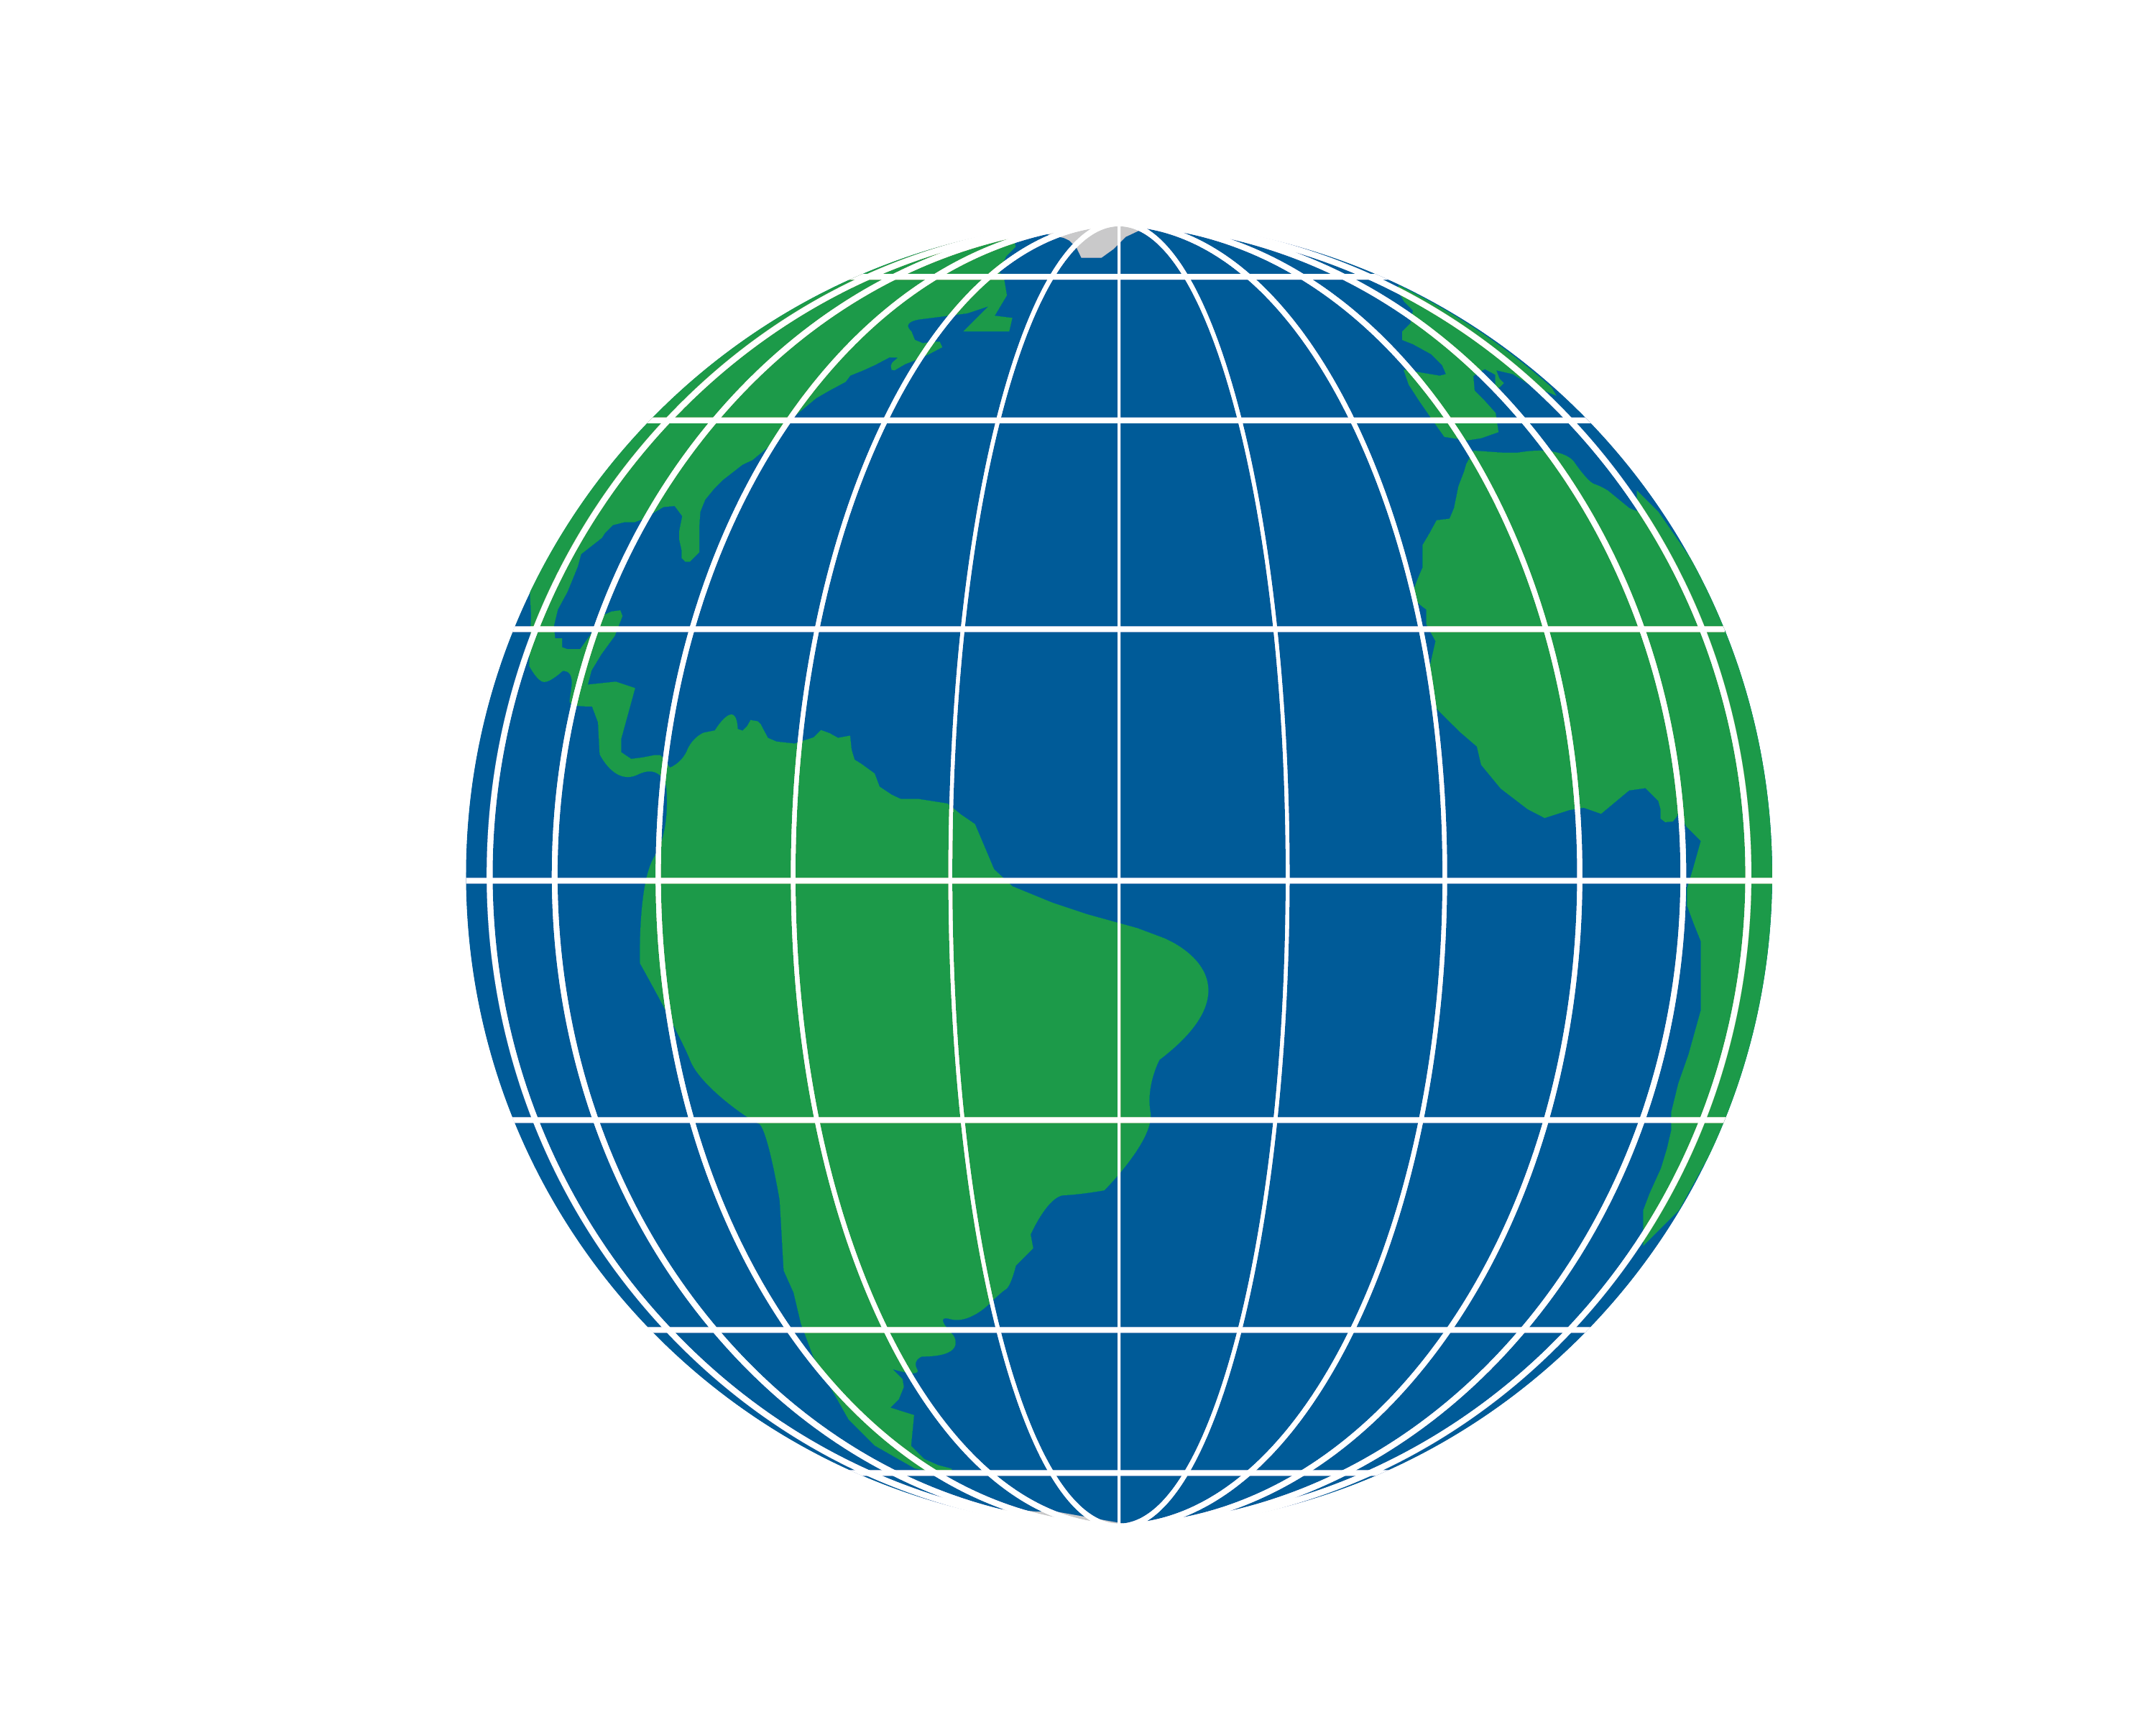
\includegraphics[width=.75\textwidth]{latLon.png}
    \caption{A diagram of latitude and longitude.}
    \label{fig:latLon}
\end{figure}

\index{latitude}
Latitude is a measure of a point's distance north or south of the
equator, expressed in degrees. It ranges from $-90^{\circ}$ at the
South Pole to $+90^{\circ}$ at the North Pole, with $0^{\circ}$
representing the Equator. (See figures~\ref{fig:latitude} and~\ref{fig:latitudeExplained})
\begin{figure}[htbp]
  \centering
  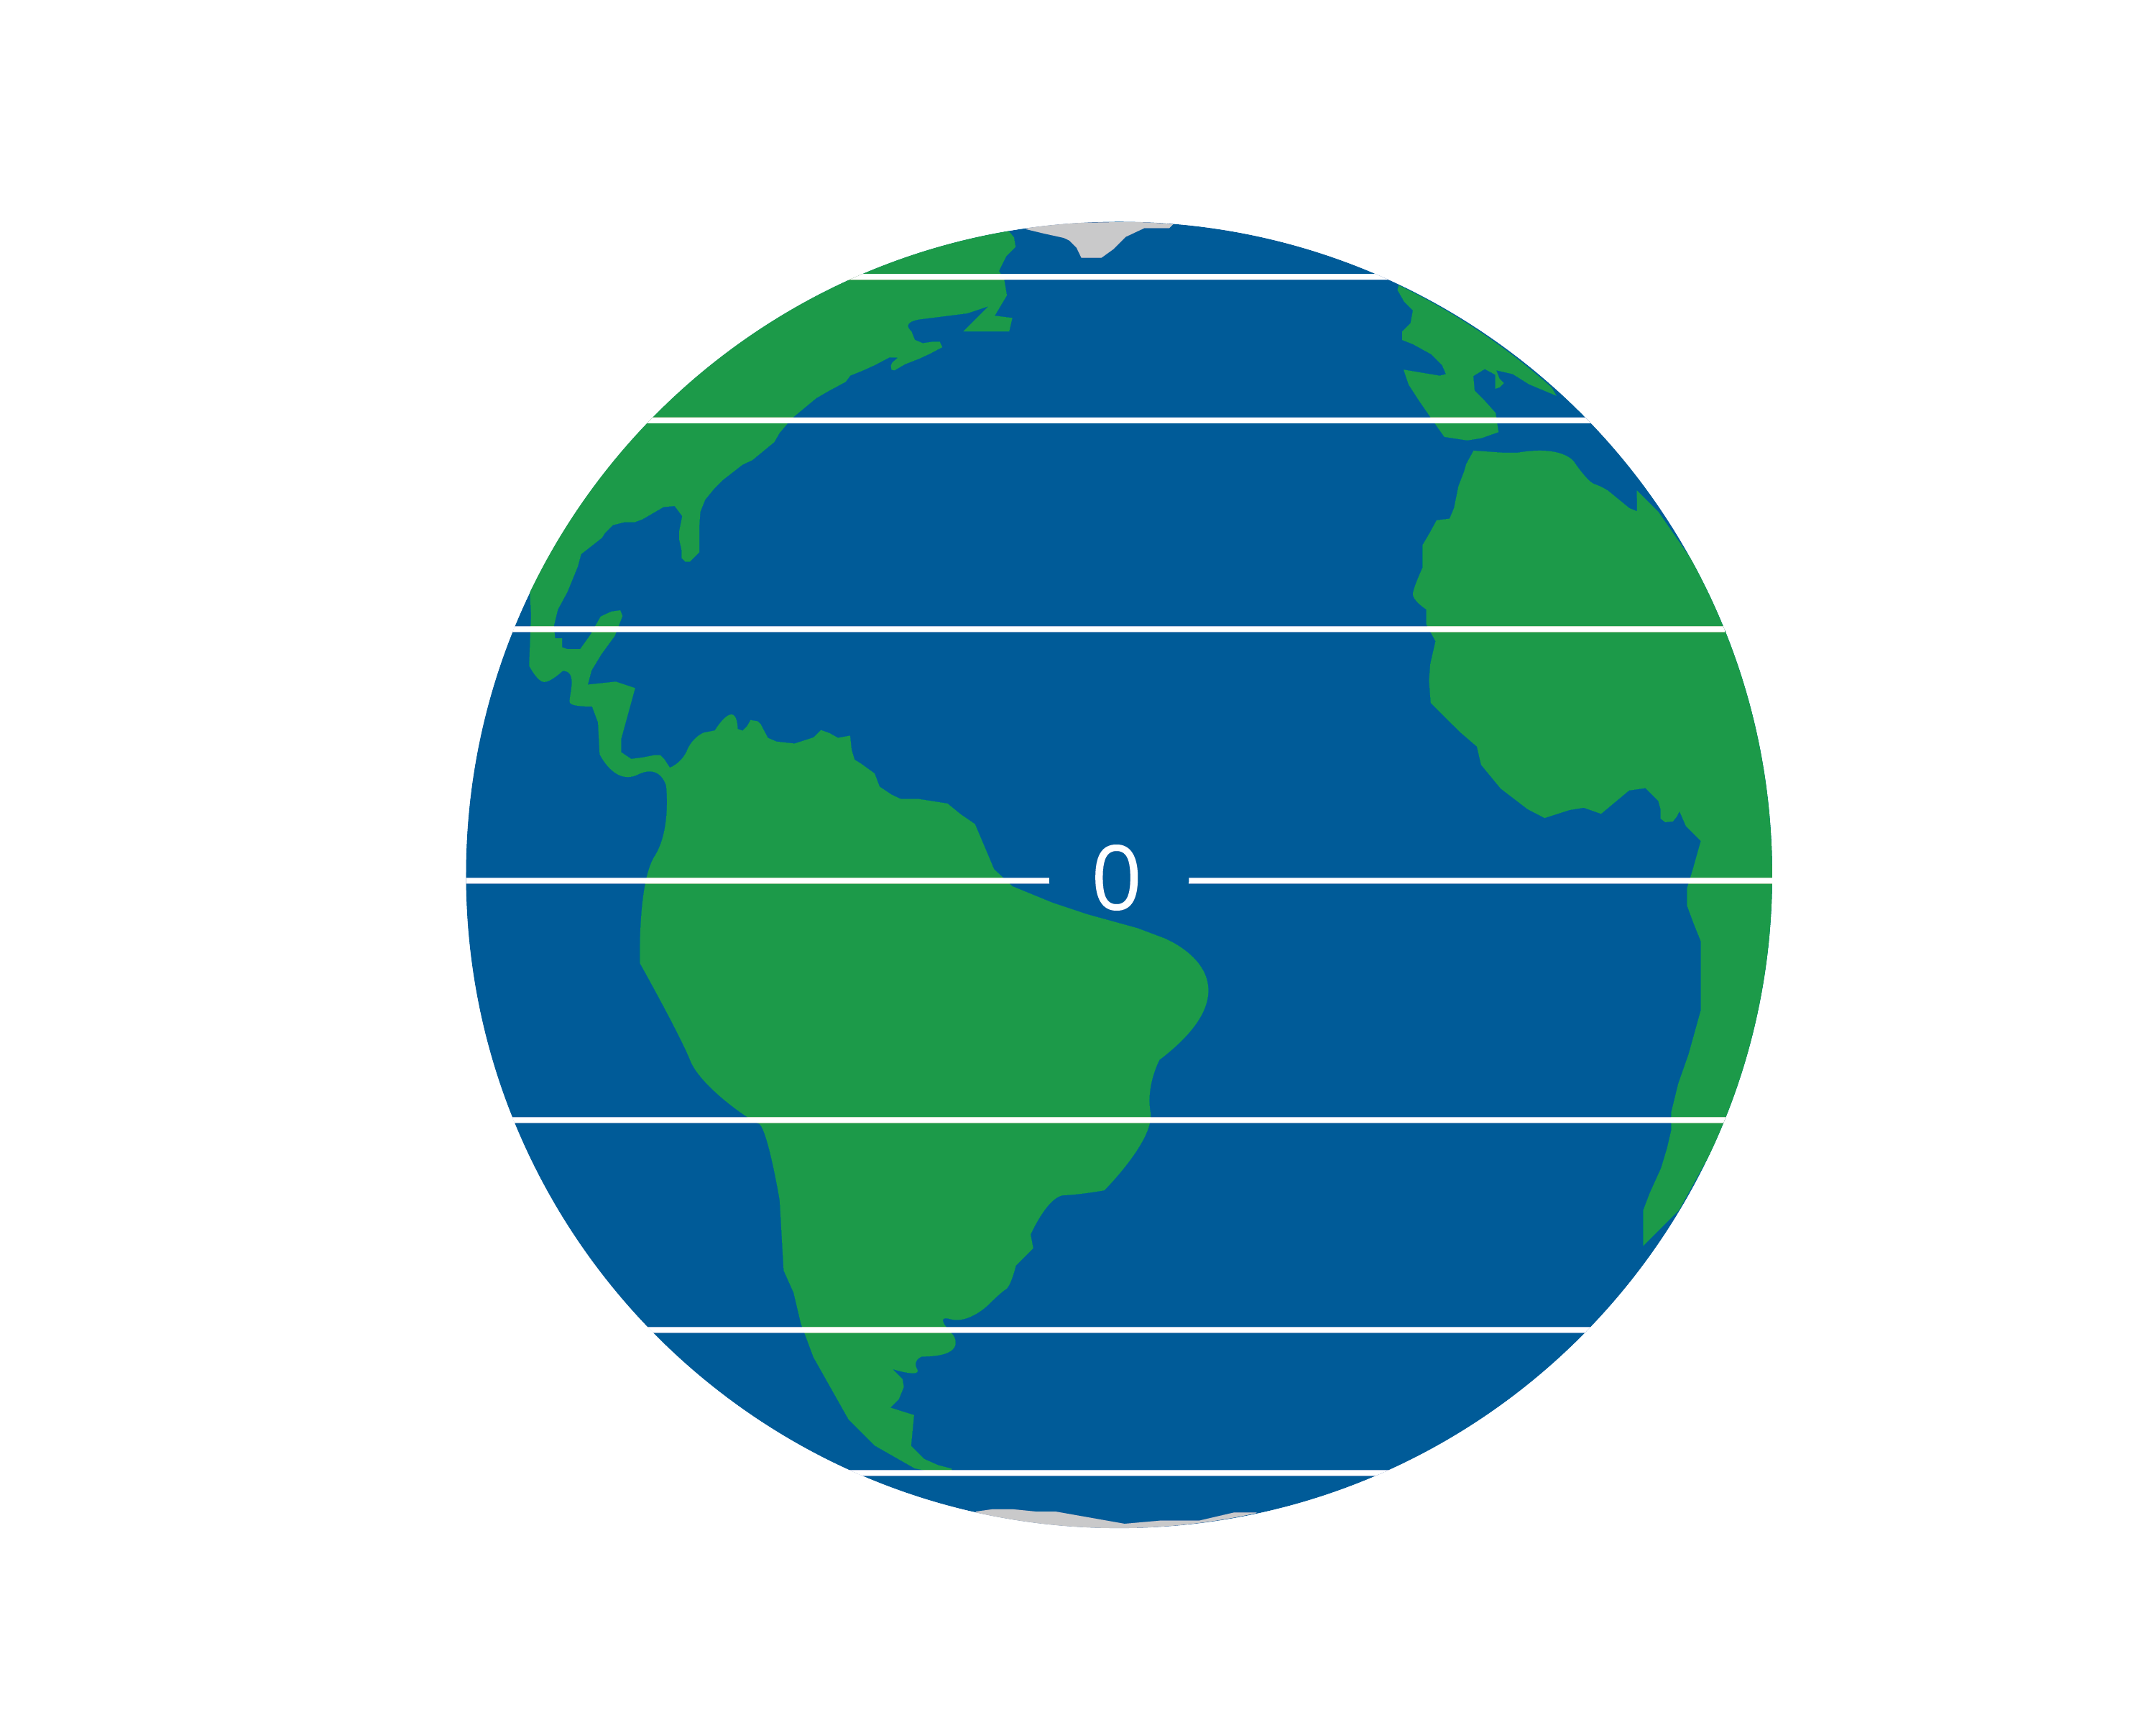
\includegraphics[width=.75\textwidth]{lat.png}
  \caption{Latitude drawn on the earth.}
  \label{fig:latitude}
\end{figure}

\begin{figure}[htbp]
  \centering
  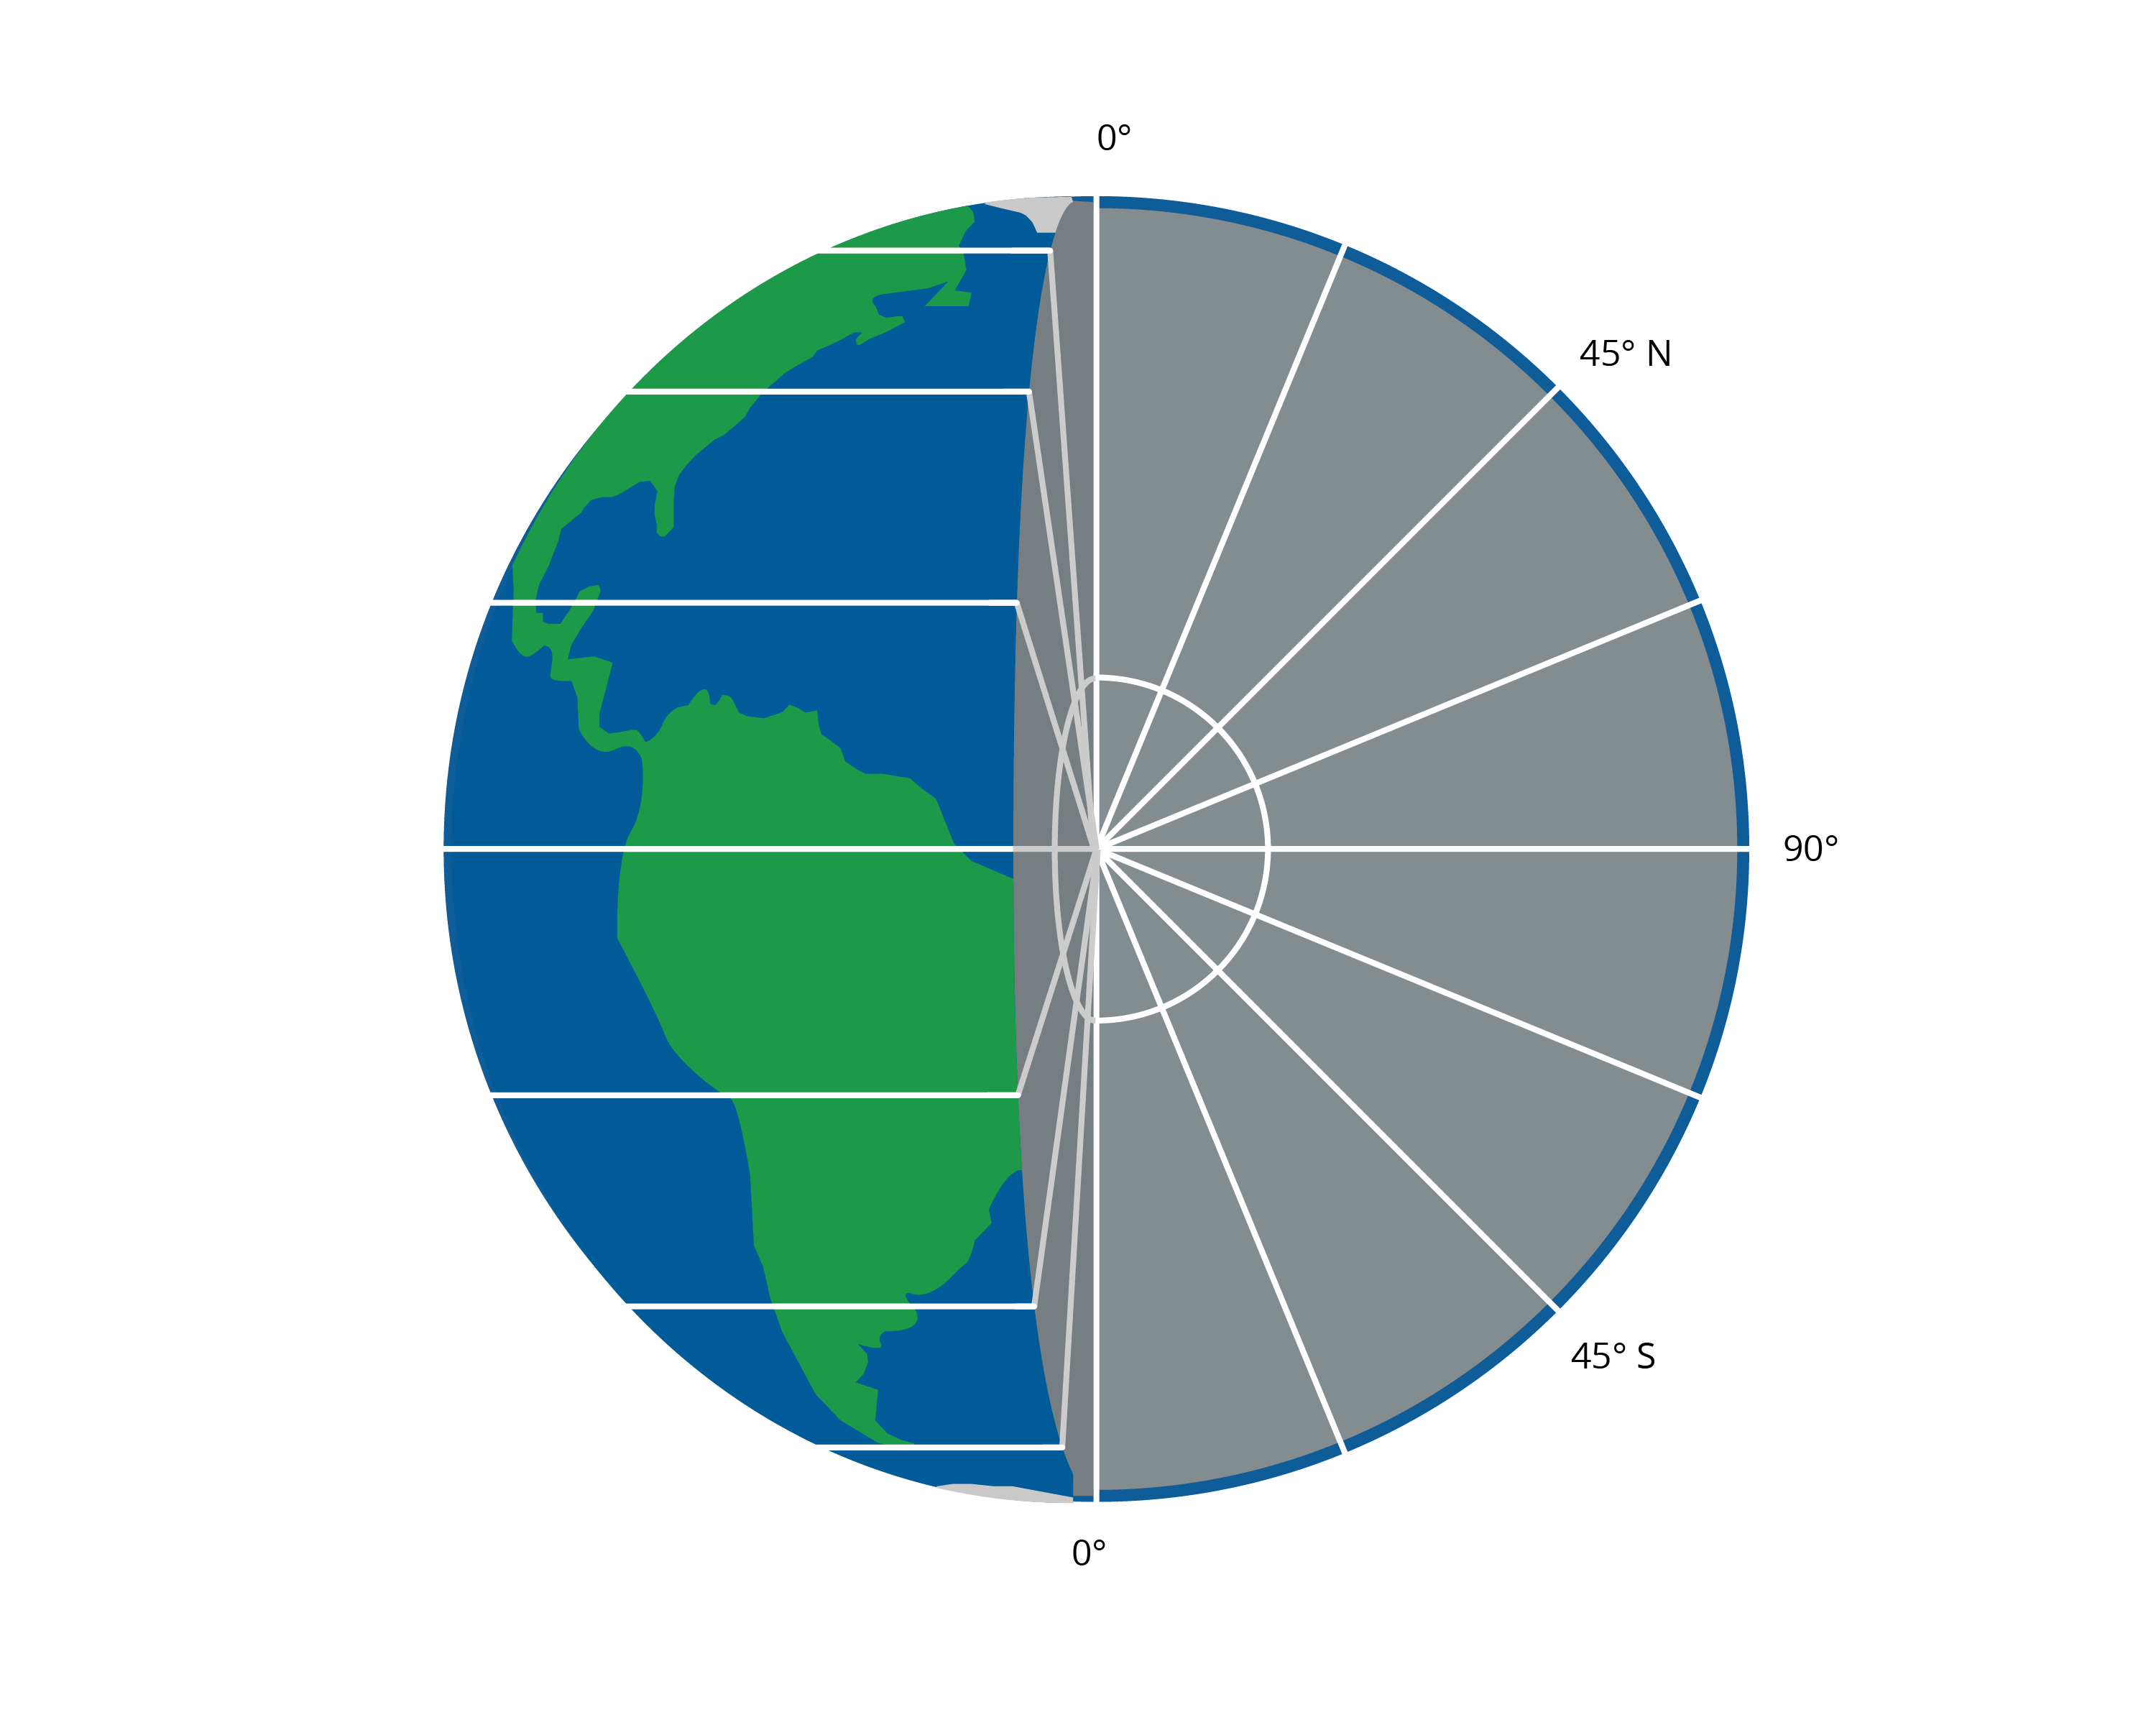
\includegraphics[width=.75\textwidth]{latExplanation.png}
  \caption{A cross-section of the earth showing latitude.}
  \label{fig:latitudeExplained}
\end{figure}
\index{longitude}
Longitude, on the other hand, measures a point's distance east or west
of the Prime Meridian (which passes through Greenwich, England). It
ranges from $-180^{\circ}$ to $+180^{\circ}$, with the Prime Meridian
represented as $0^{\circ}$. (See figures~\ref{fig:longitude} and~\ref{fig:longExplanation})

\begin{figure}[htbp]
    \centering
    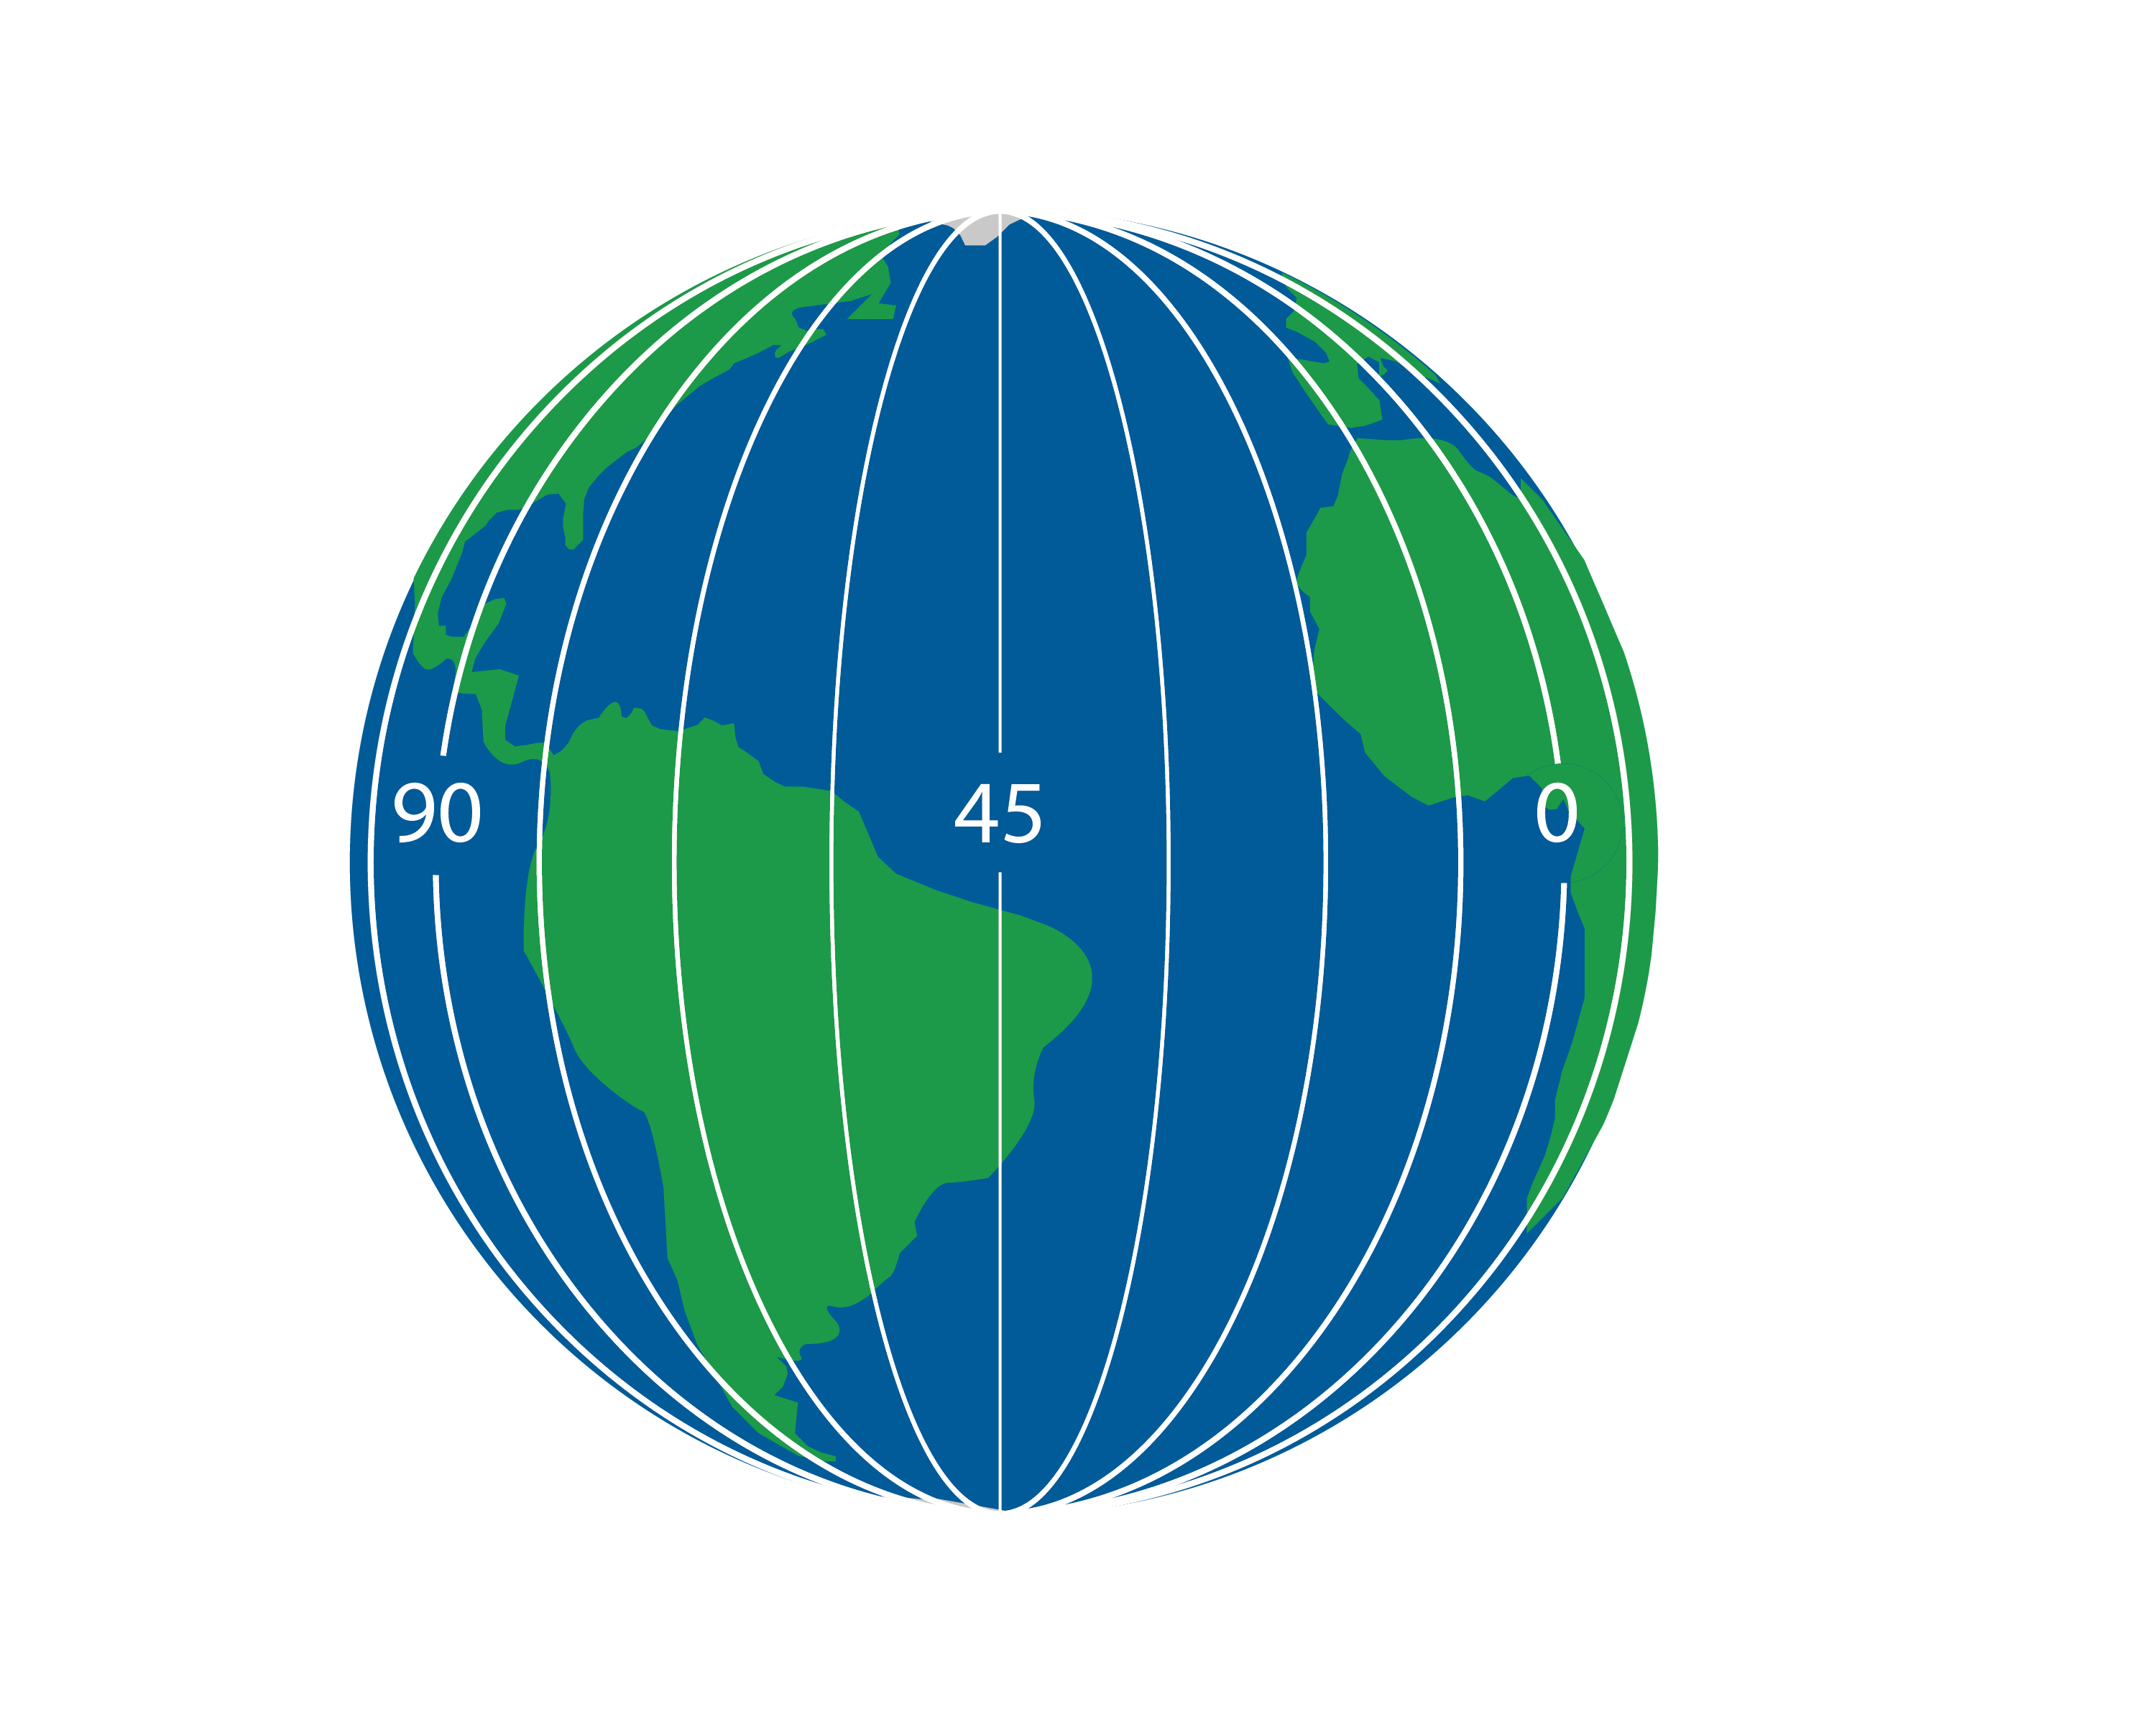
\includegraphics[width=.75\textwidth]{long.png}
    \caption{Longitudinal lines drawn on the earth.}
    \label{fig:longitude}
\end{figure}
\begin{figure}[htbp]
  \centering
  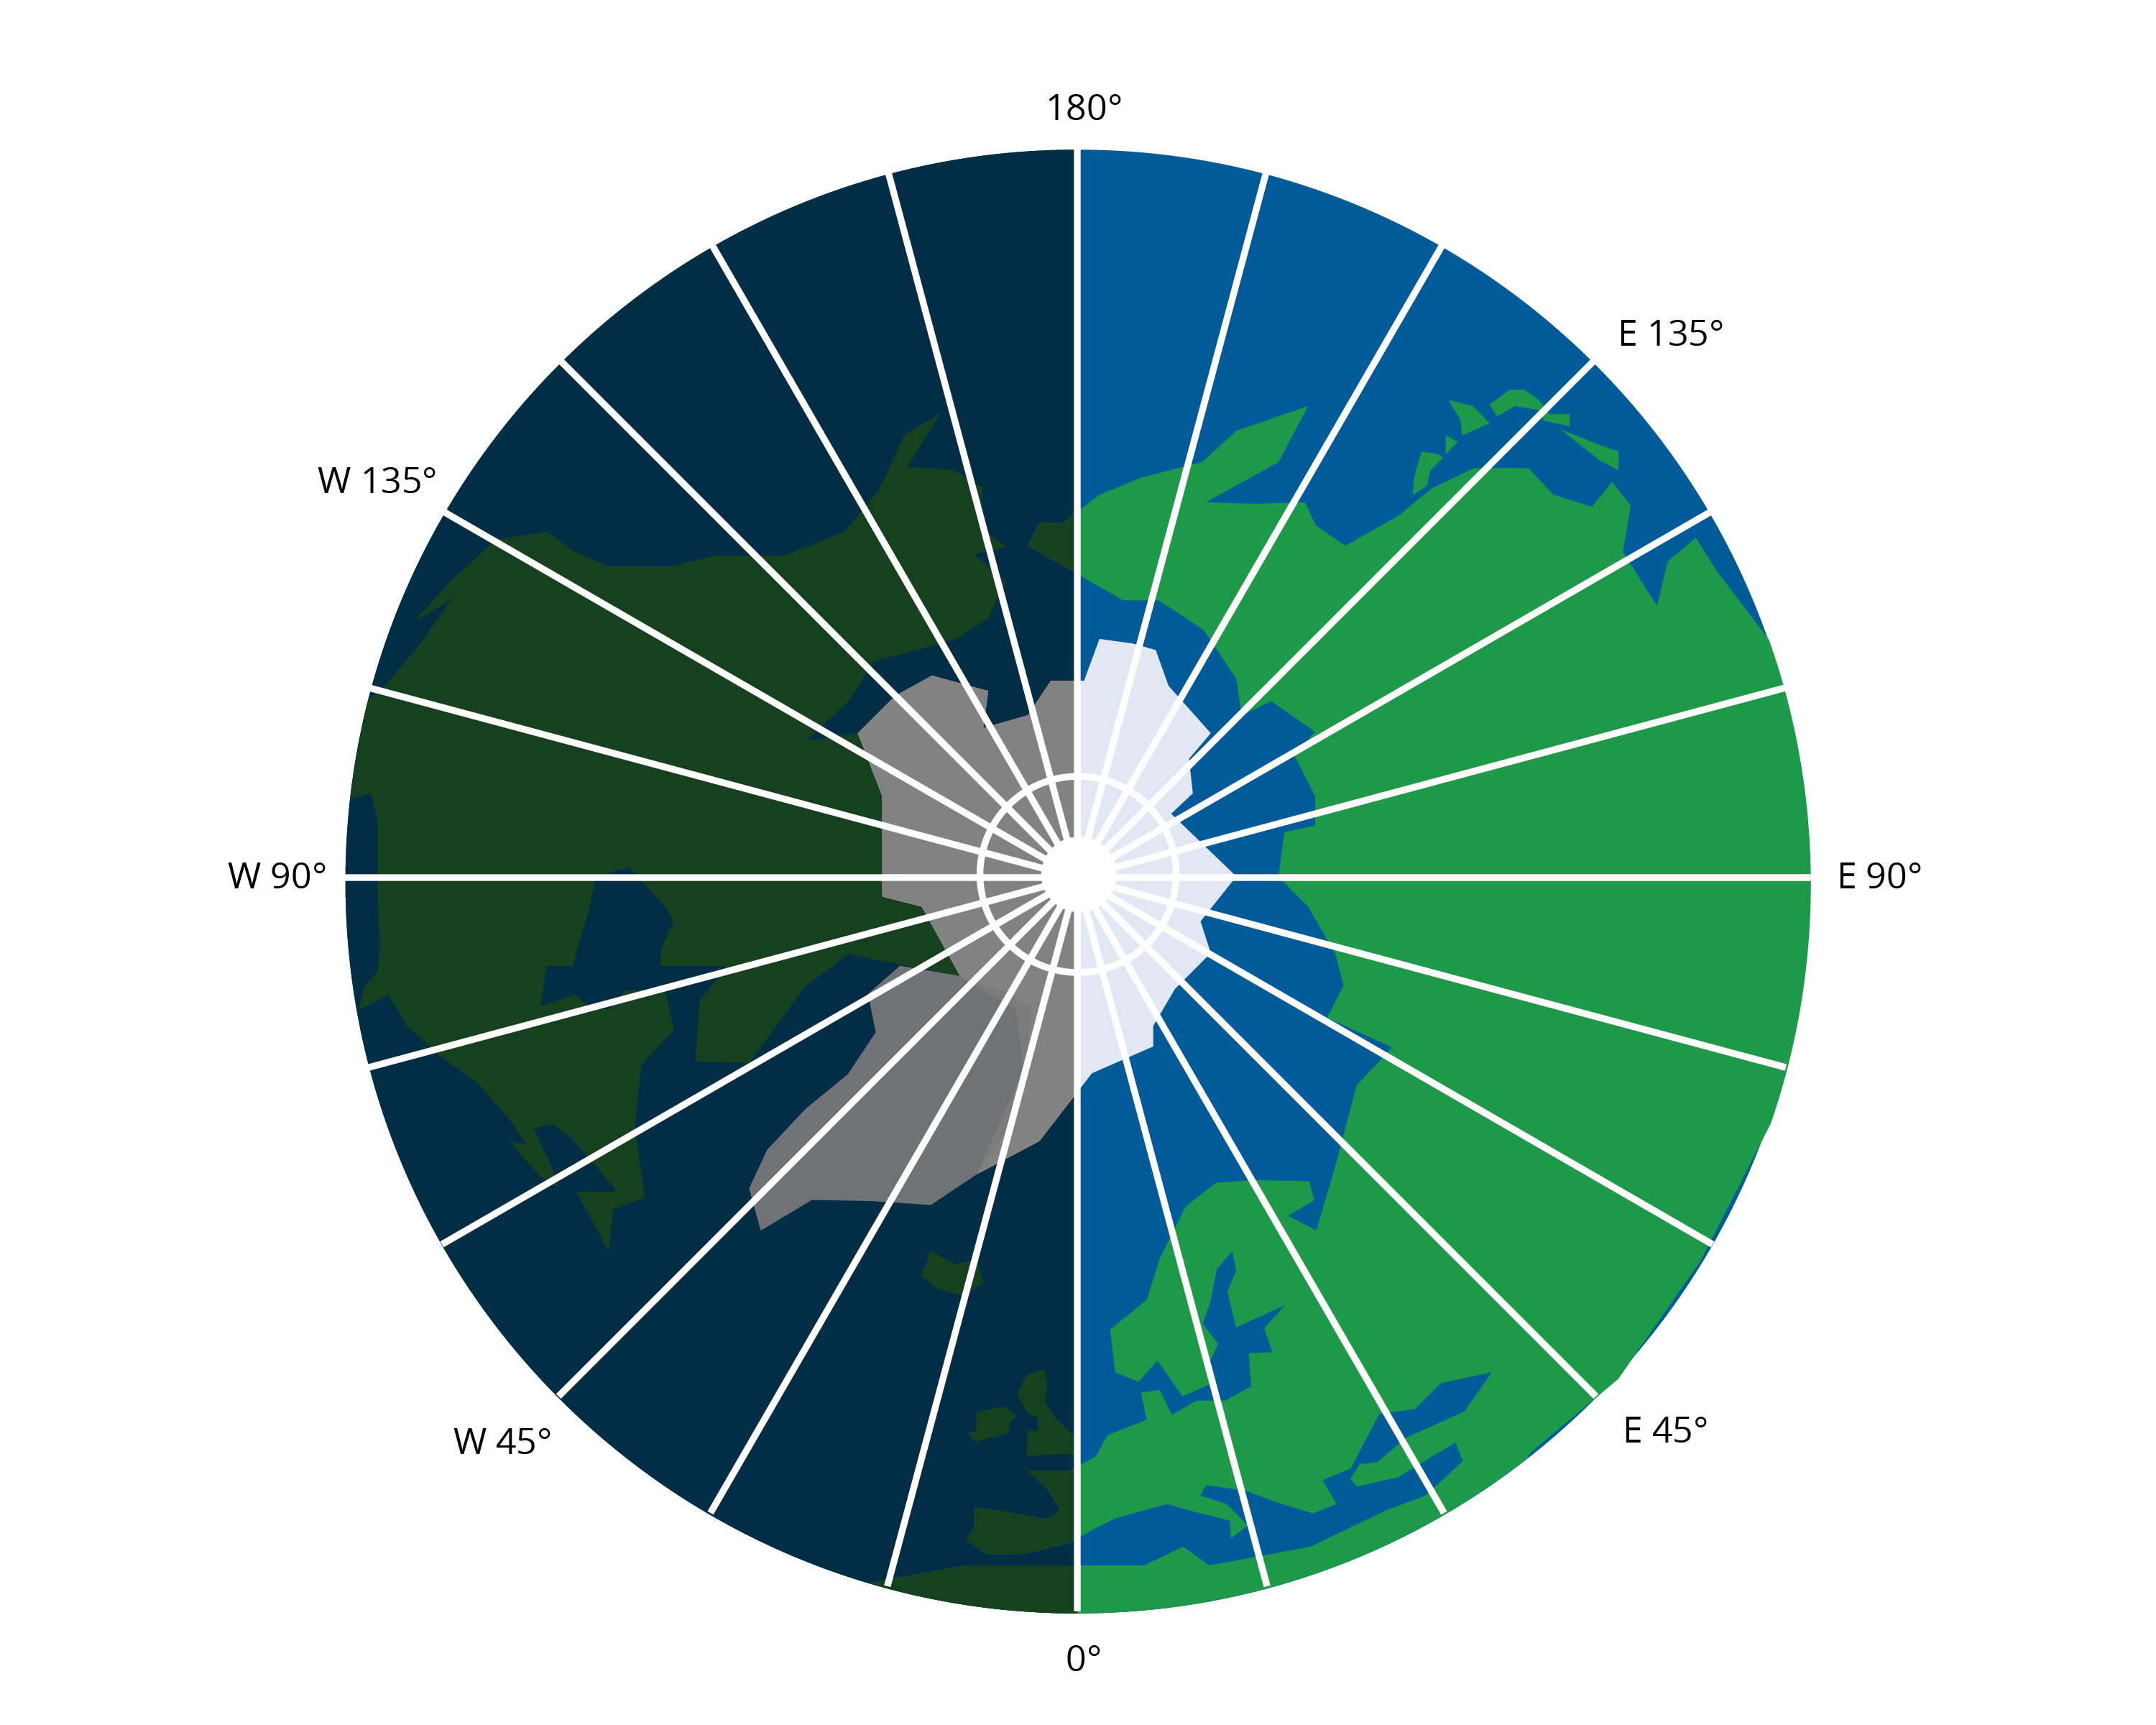
\includegraphics[width=.75\textwidth]{longExplanation.png}
    \caption{A cross-section of the earth showing longitude.}
    \label{fig:longExplanation}
\end{figure}
\index{Longitude and Latitude ! coordinates of}
The coordinates follow a system of latitude and then longitude (in the majority of contexts). Here is the Longitude and Latitude of four different large cities:
\begin{itemize}
  \item \textbf{London, England}: $51^\circ$ N $0^\circ$ W
  \item \textbf{New York City, New York, USA}: $40^\circ$ N $74^\circ$ W
  \item \textbf{Sydney, New South Whales, Australia}: $33^\circ$ S $150^\circ$ E
  \item \textbf{Rio de Janerio, Brazil}: $22^\circ$ S $43^\circ$ W
\end{itemize}

These coordinates may be broken down further into minute and second components as well, for futher geometric accuracy.
Each degree ($^\circ$) is divided into 60 minutes ($'$). Each minute ($'$) is divided into 60 seconds ($"$). Just like in time. Note some do not

\begin{itemize}
  \item \textbf{London, England}: $51^\circ$ 30` 26" N $0^\circ$ 7` 39" W
  \item \textbf{New York City, New York, USA}: $40^\circ$ 42` 46" N $74^\circ$ 0` 22" W
  \item \textbf{Sydney, New South Whales, Australia}: $33^\circ$ 52` 0" S $150^\circ$ 12` 0" E
  \item \textbf{Rio de Janerio, Brazil}: $22^\circ$ 54` 0" S $43^\circ$ 12` 0" W
\end{itemize}

\section{Nautical Mile}
\index{Nautical Mile}
A nautical mile is a unit of measurement used primarily in aviation
and maritime contexts. It is based on the circumference of the Earth,
and is defined as one minute ($1/60^{\circ}$) of latitude; in other words, \textbf{one minute of latitude is equal to 1 nautical mile.} 
This makes it directly related to the Earth's geometry, unlike a kilometer or a
mile, which are arbitrary in nature. The exact value of a nautical
mile can vary slightly depending on which type of latitude you use
(e.g., geodetic, geocentric, etc.), but for practical purposes, it is
often approximated as 1.852 kilometers or 1.15078 statute miles.\index{nautical mile}

\section{Haversine Formula}

The haversine formula is an important equation in navigation for
giving great-circle distances between two points on a sphere from
their longitudes and latitudes. It is especially useful when it comes
to calculating distances between points on the surface of the Earth,
which we represent as a sphere for simplicity. See Figure~\ref{fig:haversine} \index{Haversine formula}

\begin{figure}[htbp]
    \centering
    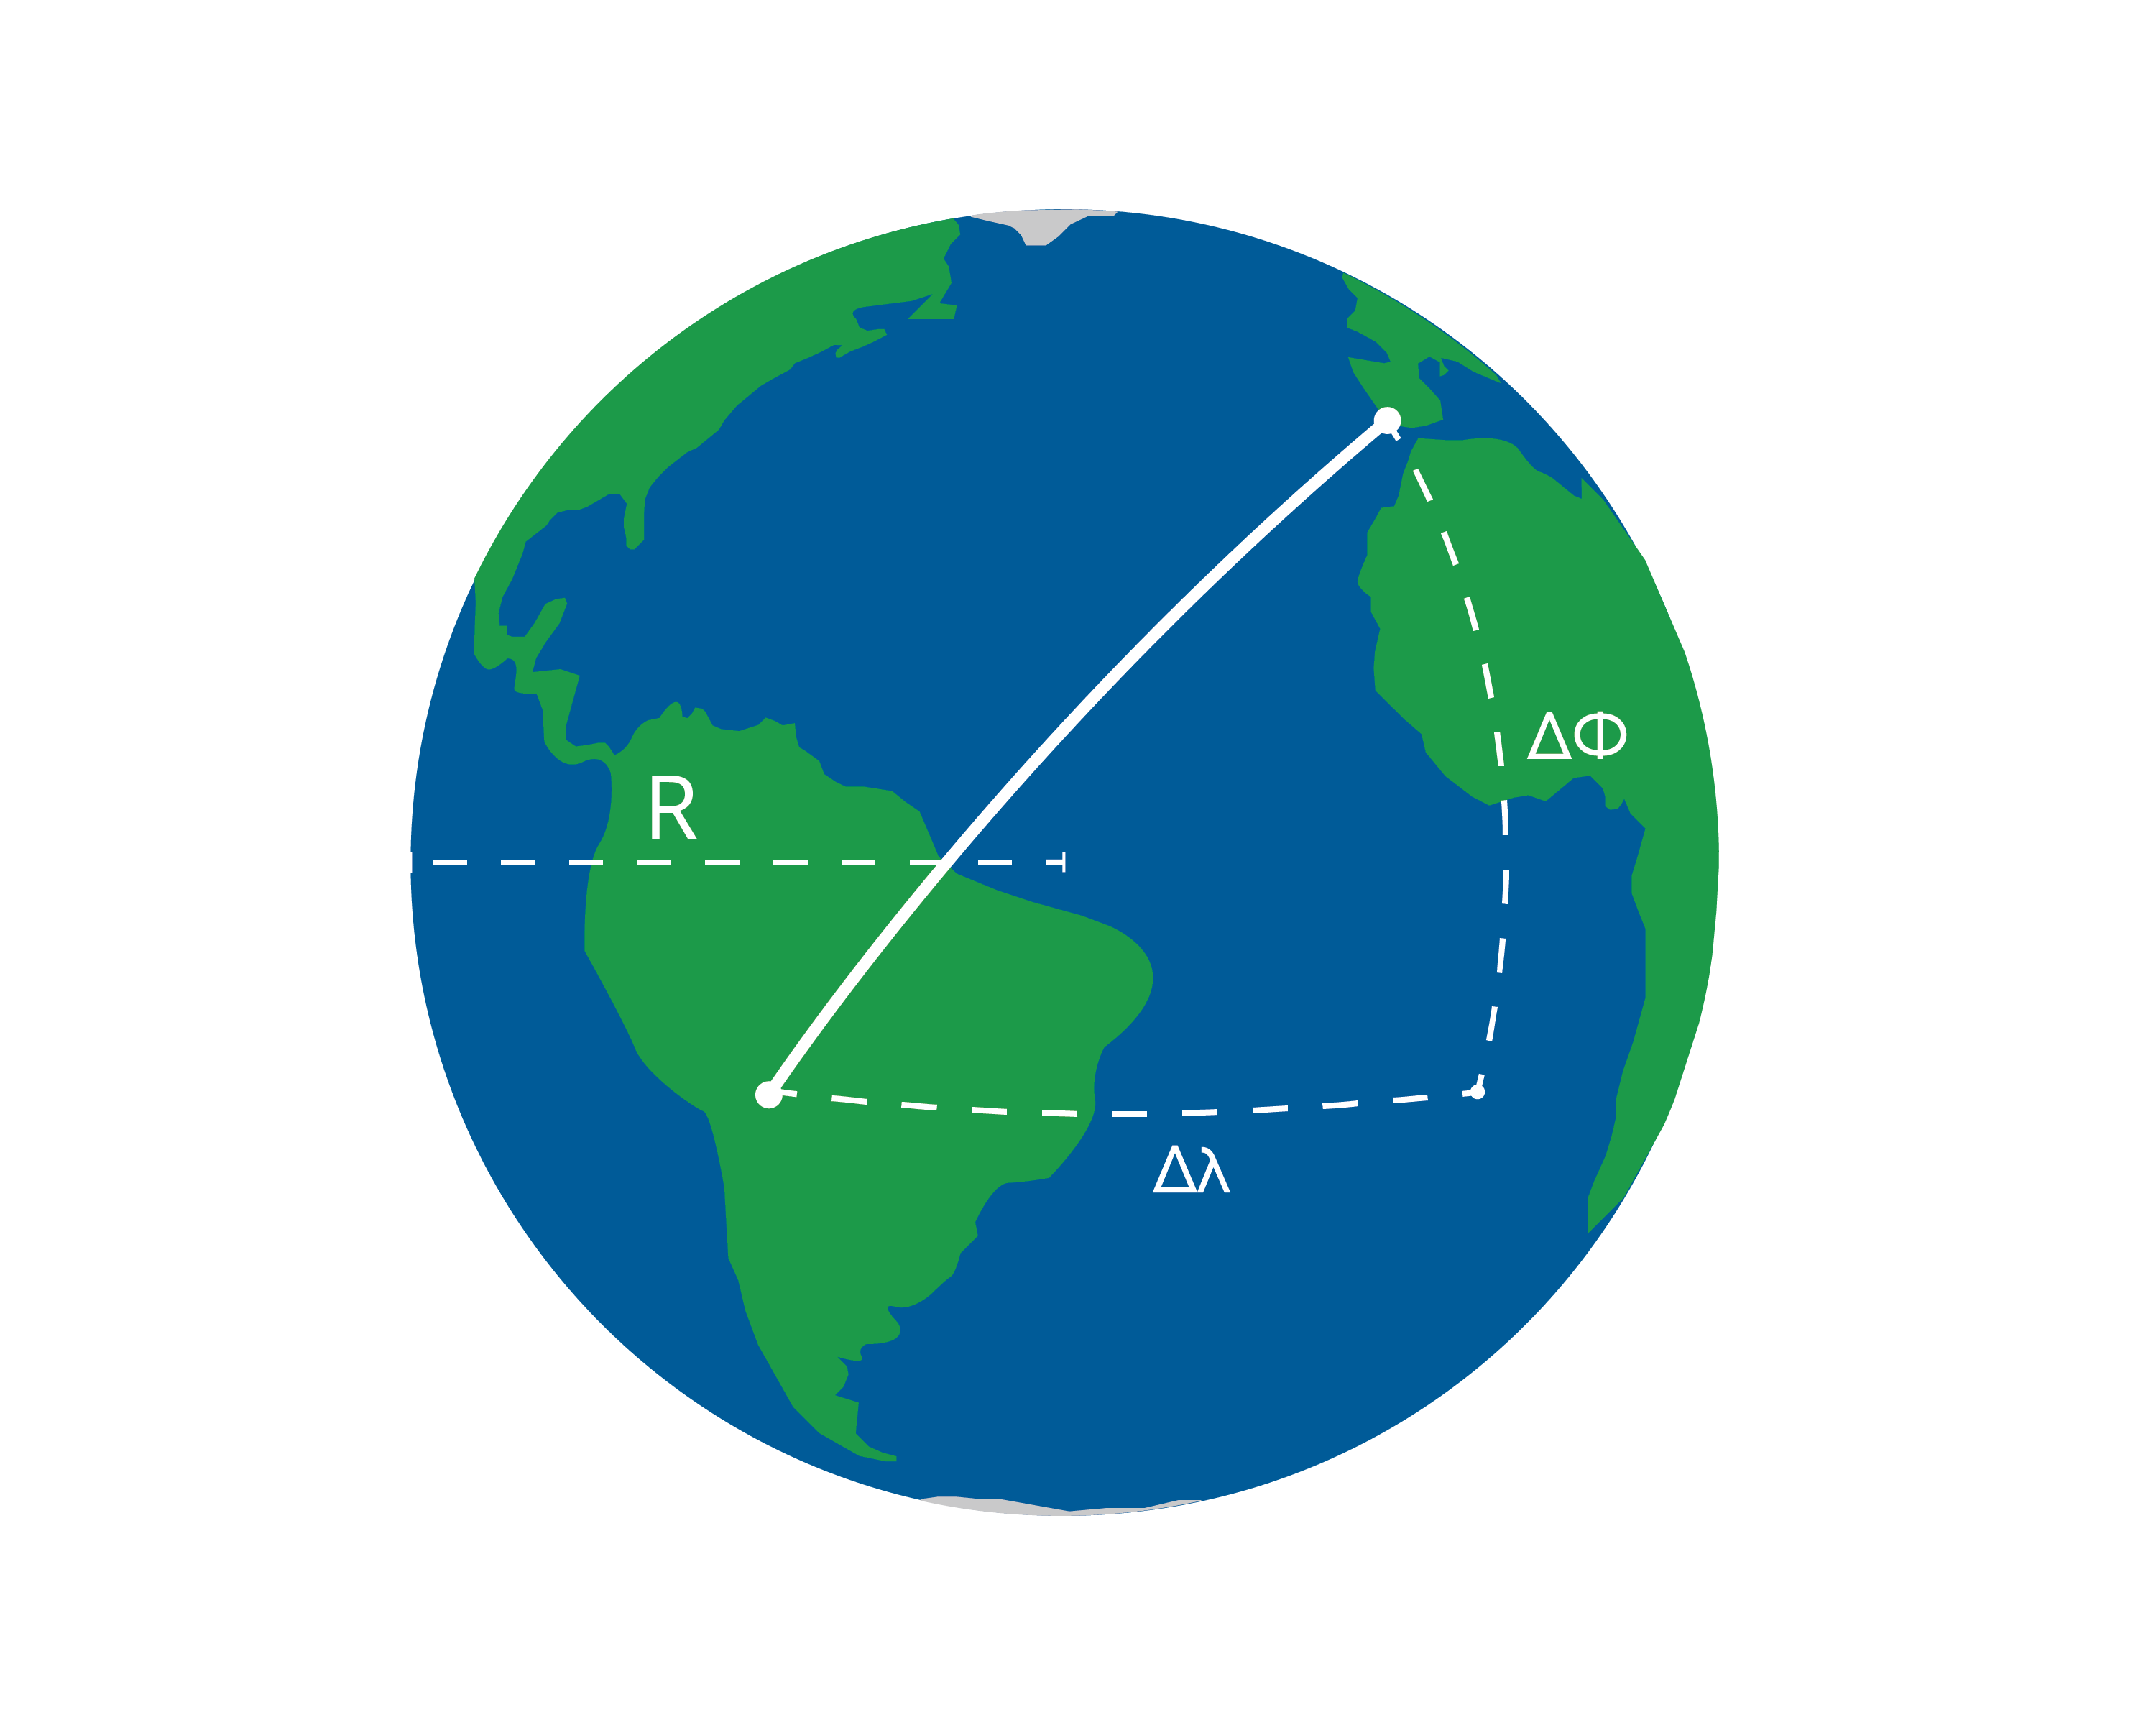
\includegraphics[width=\textwidth]{haversine.png}
    \caption{A diagram of the haversine formula.}
    \label{fig:haversine}
\end{figure}


In its basic form, the haversine formula is as follows:
%FIXME I feel like this section may need more clarification if the formula is important.

The angle found using haversine $\text{haversine}(\theta) = sin^2\left(\frac{\theta}{2}\right)$:

\[
a = \sin^2\left(\frac{\Delta\phi}{2}\right) + \cos(\phi_1)\cos(\phi_2)\sin^2\left(\frac{\Delta\lambda}{2}\right)
\]

Compute $c$ which determines the angular distance using $atan2$, a computer science tangential function with 2 arguments equivalent to $2 \arcsin(\sqrt{a})$\footnote{Note that this function is not available on calculators, but commonly used in computer science programs. You may use the singular argument equivalent in calculations.}:
\[
c = 2 \cdot \text{atan2} \left( \sqrt{a}, \sqrt{1-a} \right)
\]


Find $d$, the true distance along the sphere:

\[
d = R \cdot c
\]

In one line, this is:
$$
d = 2R \cdot \arcsin\left( \sqrt{\sin^2\left(\frac{\Delta\phi}{2}\right) + \cos(\phi_1) \cos(\phi_2) \sin^2\left(\frac{\Delta\lambda}{2}\right)} \right)
$$

Here, $\phi_1$ and $\phi_2$ represent the latitudes of the two points (in radians),
$\Delta\phi$ and $\Delta\lambda$ represent the differences in latitude
and longitude (also in radians), and $R$ is the radius of the
Earth (using whatever unit of distance you desire). The result, $d$, is the distance between the two points along
the surface of the sphere. Notice that $d$ is equal to the formula for the \emph{arc length} of a sector. 
A sphere is just a bunch of circles with radius $r$, so it follows that we can use formulas for circles in our spherical calculations. 

This is why planes fly arc-shaped paths rather than straight paths from points $A \to B$. Planes follow the shortest path between two points on a sphere, called a \emph{great-circle route}. On a map, like plane flight-progress maps or the Mercator projection, the straight path looks very arc shaped, but this is just a geographical illusion. This straight distance can be calculated using the haversine formula, ultiamtely minimizing distance and fuel using the `as-the-crow-flies' path. 

